\documentclass{article}
\usepackage{esc103}

\title{ESC103: Midterm 1 Review}
\author{QiLin Xue}
\date{Fall 2020}
\usepackage{lmodern}
\usepackage{tikz}
\usepackage{pgfplots}
\usepackage{bm}
\usepackage{textcomp}
\usepackage{graphicx}
\usepackage{bbm}
\usepackage{parskip}
\usepackage{multicol}
\usetikzlibrary{arrows}
\pgfplotsset{compat=1.16}
\setlength\parindent{0pt}
\everymath{\displaystyle}
\usepackage{makeidx}
\makeindex
\let\oldtextbf\textbf
\renewcommand{\textbf}[1]{\oldtextbf{#1}\index{#1}}


\usepackage{xstring}
\usepackage{forloop}


\begin{document}
\newcounter{idx}
\newcounter{posx}
\newcommand{\rotraise}[1]{%
  \StrLen{#1}[\slen]
  \forloop[-1]{idx}{\slen}{\value{idx}>0}{%
    \StrChar{#1}{\value{idx}}[\crtLetter]%
    \IfSubStr{tlQWERTZUIOPLKJHGFDSAYXCVBNM}{\crtLetter}
      {\raisebox{\depth}{\rotatebox{180}{\crtLetter}}}
      {\raisebox{1ex}{\rotatebox{180}{\crtLetter}}}}%
}

\maketitle
\tableofcontents
\printindex
\newpage
\section{Basic Vectors}
The \textbf{linear combination} of vectors $\vec{v}$ and $\vec{w}$ is given by:
\begin{equation}
    c\vec{v}+d\vec{w}
    \label{eq:}
\end{equation}
where $c$ and $d$ are scalars. Note that \textbf{vector addition} is both \textbf{associative} and \textbf{commutative.}

The length of a vector in $\vec{v}$ in $\mathbb{R}^N$ is given by:
\begin{equation}
    \lVert v\rVert = \sqrt{v_1^2+v_2^2+\cdots+V_N^2}
    \label{eq:}
\end{equation}
The \textbf{dot product} (also known as scalar product) is defined as:
\begin{equation}
    \vec{v}\cdot\vec{w} = v_1w_1+v_2w_2+v_3w_3+\cdots+v_Nw_N
    \label{eq:}
\end{equation}
for two vectors $\vec{v}$ and $\vec{w}$ in $\mathbb{R}^N$. Using these, we can derive the following ideas and theorems.
\begin{idea}
    The dot product of a vector with itself gives the square of its length:
    \begin{equation}
        \lVert \vec{v}\rVert ^2 = \vec{v}\cdot \vec{v}
        \label{eq:}
    \end{equation}
\end{idea}
\begin{idea}
    The \textbf{angle between two vectors} is given by:
    \begin{equation}
        \cos\theta = \frac{\vec{w}\cdot\vec{v}}{\lVert \vec{w}\rVert \lVert \vec{v} \rVert}
    \end{equation}
\end{idea}
\begin{idea}
    The \textbf{triangle inequality} is:
    \begin{equation}
        \lVert \vec{v}+\vec{w} \rVert \le \lVert\vec{v}\rVert + \lVert\vec{v}\rVert
        \label{eq:}
    \end{equation}
\end{idea}
\begin{idea}
    The \textbf{Cauchy-Schwarz-Bunakowsky Inequality} is:
    \begin{equation}
        |\vec{v}\cdot\vec{w}| \le \lVert\vec{v}\rVert \lVert\vec{w}\rVert
        \label{eq:}
    \end{equation}
\end{idea}
\begin{idea}
    The \textbf{projection} of $\vec{w}$ on $\vec{v}$ can be written as:
    \begin{equation}
        \vec{u}=\text{proj}_{\vec{v}}\vec{w}=\frac{\vec{w}\cdot\vec{v}}{\lVert \vec{v} \rVert^2}\vec{v} = \frac{\vec{w}\cdot\vec{v}}{\lVert\vec{v}\rVert}\frac{\vec{v}}{\lVert\vec{v}\rVert}
        \label{eq:}
    \end{equation}
    You can view the last part $\frac{\vec{v}}{\lVert \vec{v}\rVert}$ as a unit vector pointing in the direction of $\vec{v}$ such that the \textbf{scalar projection} can be defined as:
    \begin{equation}
        |\vec{u}| = |\text{proj}_{\vec{v}}\vec{w}| = \left|\frac{\vec{w}\cdot\vec{v}}{\lVert \vec{v}\rVert}\right|
        \label{eq:}
    \end{equation}
\end{idea}
\section{Plane Geometry}
The \textbf{cross product} is defined as:
\begin{equation}
    \vec{u}=\vec{v}\times \vec{w}=
    \begin{bmatrix}
        v_2w_3-v_3w_2 \\ 
        v_3w_1-v_1w_3 \\ 
        v_1w_2-v_2w_1
    \end{bmatrix}
\end{equation}
which has a magnitude of $\lVert \vec{u}\times\vec{w}\rVert = \lVert \vec{u}\rVert \lVert \vec{w}\rVert \sin\theta$. The direction can be determined using the \textbf{right hand rule}. Cross products have the following properties:
\begin{property}
    The properties of a cross product is as follows.
    \begin{itemize}
        \item Consider $3$ vectors, $\vec{v}$, $\vec{w}$, and $\vec{z}$. Then:
        \begin{equation}
            \vec{v}\times (\vec{w}+\vec{z}) = \vec{v} \times \vec{w} + \vec{v} \times \vec{z}
            \label{eq:}
        \end{equation}
        \item The cross product is not commutative, but they are anti-commutative:
        \begin{equation}
            \vec{v}\times \vec{w} = -\vec{w}\times \vec{v}
            \label{eq:}
        \end{equation}
        \item When crossed with the zero vector, we have:
        \begin{equation}
            \vec{v}\times \vec{0} = \vec{0}\times \vec{v} = \vec{0}
            \label{eq:}
        \end{equation}
        \item When multiplied by a scalar,
        \begin{equation}
            c(\vec{v}\times\vec{w}) = (c\vec{v})\times \vec{w} = \vec{v}\times (c\vec{w})
            \label{eq:}
        \end{equation}
    \end{itemize}
\end{property}
We can write out any point on a plane given a linear combination of two vectors $\vec{d}_1$ and $\vec{d}_2$ which span the plane:
\begin{equation}
    \begin{bmatrix}
        x\\y\\z
    \end{bmatrix}=\begin{bmatrix}
        x_0\\y_0\\z_0
    \end{bmatrix}+c\vec{d}_1+d\vec{d}_2
    \label{eq:}
\end{equation}
where $\begin{bmatrix}
    x_0\\y_0\\z_0
\end{bmatrix}$ is any known point on the plane. Additionally, we can define a plane by its normal vector:
\begin{equation}
    \vec{n}=\begin{bmatrix}
        a\\b\\c
    \end{bmatrix}
    \label{eq:}
\end{equation}
by taking the cross product between any two vectors $\overrightarrow{P_0P}$ that lie on the plane such that:
\begin{equation}
    \overrightarrow{P_0P} \cdot \vec{n} = 0
    \label{eq:}
\end{equation}
Using this information, we can derive the following theorems and ideas:
\begin{idea}
    If $\vec{n}=\begin{bmatrix}
        a\\b\\c
    \end{bmatrix}$ is a normal vector, then the plane that it defines can be represented by the \textbf{scalar equation} $ax+by+cz+d=0$.
    \begin{proof}
        Suppose we know a given point $P_0=\begin{bmatrix}
            x_0\\y_0\\z_0
        \end{bmatrix}$ on the plane. Then we can choose any other point on the plane $P=\begin{bmatrix}
            x\\y\\z
        \end{bmatrix}$ which can define any arbitrary vector that is paralell to the plane:
        \begin{equation}
            \vec{v} = P-P_0 = \begin{bmatrix}
                x-x_0\\y-y_0\\z-z_0
            \end{bmatrix}
            \label{eq:}
        \end{equation}
        The dot product between $\vec{v}$ and $\vec{n}$ must be equal to zero, which gives:
        \begin{equation}
            a(x-x_0)+b(y-y_0)+c(z-z_0)=0
            \label{eq:}
        \end{equation}
        Expanding, we get the form that we desire.
    \end{proof}
\end{idea}
\begin{idea}
    The distance from a point $P=(x_0,y_0,z_0)$ to the plane $ax+by+cz+d=0$ is given by:
    \begin{equation}
        D = \frac{|ax_0+by_0+cz_0+d|}{\sqrt{a^2+b^2+c^2}}
        \label{eq:}
    \end{equation}
    \textit{Note:} We are not allowed to use this formula on the test, but we can derive it below. Refer to the following diagram:
\begin{center}
    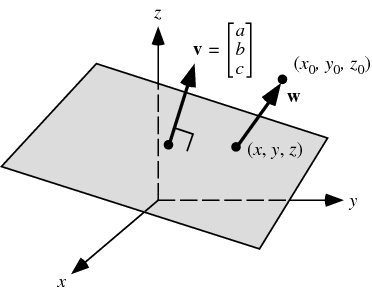
\includegraphics[width=0.4\linewidth]{plane-point.png}
\end{center}
    \begin{proof}
        The normal vector to the plane is given by:
        \begin{equation}
            \vec{n}=\begin{bmatrix}
                a\\b\\c
            \end{bmatrix}
            \label{eq:}
        \end{equation}
        
        Define $\vec{w}$ as the vector from any point $P$ to any given point $(x,y,z)$ on the plane such that:
        \begin{equation}
            \vec{w} = \begin{bmatrix}
                x-x_0\\ 
                y-y_0 \\ 
                z-z_0
            \end{bmatrix}
            \label{eq:}
        \end{equation}
        The scalar projection of $\vec{w}$ on $\vec{n}$ then gives the orthogonal component, and thus the shortest distance between $P$ and the plane:
        \begin{align}
            D &= |\text{proj}_{\vec{n}}\vec{w}| \\ 
            &= \frac{|\vec{n}\cdot\vec{w}|}{|\vec{v}|} \\ 
            &=
             \left|\frac{a(x-x_0)+b(y-y_0)+c(z-z_0)}{\sqrt{a^2+b^2+c^2}}\right| \\ 
             &= \left|\frac{(ax+by+cz)-ax_0-by_0-cz_0}{\sqrt{a^2+b^2+c^2}}\right| \\ 
             &= \left|\frac{-d-ax_0-by_0-cz_0}{\sqrt{a^2+b^2+c^2}}\right| \\ 
             &= \left|\frac{d+ax_0+by_0+cz_0}{\sqrt{a^2+b^2+c^2}}\right|
        \end{align}
    \end{proof}
    This is the general way when determining the distance from a point to a plane. You first need to figure out the normal vector (e.g. this can also be done by determining two vectors that lie parallel to the plane and taking their cross product), and then the vector between any given point to the point of interest. Getting the orthogonal projection yields the distance to the plane.
\end{idea}
\begin{idea}
    The projection of a vector $\vec{v}$ onto a plane $\Pi$ defined by the normal vector $\vec{n}$ is:
    \begin{equation}
        \text{proj}_{\Pi} = \vec{v}-\text{proj}_{\vec{n}}\vec{v}
        \label{eq:}
    \end{equation}
    We can also show this by drawing a picture!
\end{idea}
\section{Matrix Multiplication and Linear Transformations}
A matrix can be used to represent systems of linear equations. For example, the following set:
\begin{align}
    x-2y&=1 \\ 
    3x+2y&=11
\end{align}
can be represented by a \textbf{row picture}, which represents the classical ``find the intersection'' visual approach. It can also be represented via a \textbf{column picture}:
\begin{equation}
    x\begin{bmatrix}
        1\\3
    \end{bmatrix}
    +y\begin{bmatrix}
    -2\\2
    \end{bmatrix}=\begin{bmatrix}
        1\\11
    \end{bmatrix}
    \label{eq:}
\end{equation}
It can also be represented via matrices:
\begin{equation}
    \underbrace{\begin{bmatrix}
        1&-2\\3&2
    \end{bmatrix}}_\text{Matrix A}\underbrace{\begin{bmatrix}
        x\\y
    \end{bmatrix}}_{\text{vector } \vec{x}}=\underbrace{\begin{bmatrix}
        1\\11
    \end{bmatrix}}_{\text{vector }\vec{b}}
\end{equation}
We can perform \textbf{matrix multiplication} if $A$ has $n$ columns and $B$ has $n$ rows.
\begin{idea}
    hen multiplying two matrices, the entry in row $i$ and column $j$ of $AB$ is:
    \begin{equation}
        \text{(Row i of A)} \cdot \text{(column j of B)}
    \end{equation}
    Recall that $A$ and $B$ can only be multiplied of $A$ is $m\times n$ and $B$ is $n\times p$. The size of the resulting matrix is therefore $m\times p$.
\end{idea}
\begin{property}
    \begin{enumerate}
        \item $A+B=B+A$ (commutative)
        \item $c(A+B)=cA+cB$ (where $c$ is scalar)
        \item $A+(B+C)=(A+B)+C$ (associative)
        \item $C(A+B)=CA+CB$ (distributive from left)
        \item $(A+B)C=AC+BC$ (distributive from right)
        \item $A(BC)=(AB)C$ (associative)
    \end{enumerate}
\end{property}
Matrices can also be viewed as \textbf{linear transformations}. $L$ represents a linear operator iff:
\begin{enumerate}
    \item $L(c\vec{v})=cL(\vec{v})$
    \item $L(\vec{v}+\vec{w})=L(\vec{v})+L(\vec{w})$
\end{enumerate}
\begin{idea}
    All linear transformations can be summarized by matrices and represented by matrix multiplication of a vector. We can determine the matrix associated with the transformation by analyzing what happens to the unit vectors $\vec{i}$, $\vec{j}$, and $\vec{k}$, under the transformation.
\end{idea}
Using the above information, we can show the following ideas:
\begin{idea}
    The \textbf{projection} of vector $\vec{w}$ on $\vec{v}$ can be written using the linear transformation $T_2$ such that:
    \begin{equation}
        \vec{u}=T_2(\vec{w}) = \frac{1}{v_1^2+v_2^2+v_3^2}\begin{bmatrix}
            v_1^2 & v_1v_2 & v_1v_3 \\ 
            v_2v_1 & v_2^2 & v_2v_3 \\ 
            v_3v_1 & v_3v_2 & v_3^2
        \end{bmatrix}\begin{bmatrix}
            w_1\\w_2\\w_3
        \end{bmatrix}
    \end{equation}
\end{idea}
\begin{idea}
    The \textbf{identity} matrix:
        \begin{equation}
            I(\vec{w})=\vec{w}
            \label{eq:}
        \end{equation}
        where:
        \begin{equation}
            I=\begin{bmatrix}
                1&0&0\\ 
                0&1&0\\ 
                0&0&1
            \end{bmatrix}
            \label{eq:}
        \end{equation}
\end{idea}
\begin{idea}
    Suppose we have a transformation $T_1$ and $T_2$, we can define a \textbf{composition} of these transformations as:
    \begin{equation}
        T_3(\vec{v})=T_2(T_1(\vec{v})) = M_{T_2}M_{T_1}\vec{v}=M_{T_3}
        \label{eq:}
    \end{equation}
    where $M$ represents the matrix associated with the linear transformations.
\end{idea}
\begin{idea}
    We want to derive the \textbf{double angle} formulas with matrix multiplication. Suppose we wish to determine the matrix associated with the transformation of rotating a vector by an angle $\theta$ counterclockwise. We think about where the $\vec{i}$ and $\vec{j}$ vectors go to, which are $\begin{bmatrix}
        \cos\theta \\ \sin\theta
    \end{bmatrix}$ and $\begin{bmatrix}
        -\sin\theta \\ \cos\theta
    \end{bmatrix}$ respectively, so the matrix associated with it is thus:
    \begin{equation}
        M_{T_\theta} = \begin{bmatrix}
            \cos\theta & -\sin\theta \\ 
            \sin\theta & \cos\theta
        \end{bmatrix}
    \end{equation}
    which is known as the \textbf{rotation} matrix. So rotating an angle by $2\theta$ is equivalent to applying the transformation $T_\theta(T_\theta(\vec{v}))$:
    \begin{equation}
        M_{T_\theta}^2 = \begin{bmatrix}
            \cos2\theta & -\sin2\theta \\ 
            \sin2\theta & \cos2\theta
        \end{bmatrix} = \begin{bmatrix}
            \cos\theta & -\sin\theta \\ 
            \sin\theta & \cos\theta
        \end{bmatrix}\begin{bmatrix}
            \cos\theta & -\sin\theta \\ 
            \sin\theta & \cos\theta
        \end{bmatrix}
        \label{eq:}
    \end{equation}
    or:
    \begin{equation}
        \begin{bmatrix}
            \cos2\theta & -\sin2\theta \\ 
            \sin2\theta & \cos2\theta
        \end{bmatrix} = \begin{bmatrix}
            \cos^2\theta-\sin^2\theta & -2\sin\theta\cos\theta \\ 
            2\sin\theta\cos\theta & \cos^2\theta-\sin^2\theta
        \end{bmatrix}
        \label{eq:}
    \end{equation}
\end{idea}
\section{Eigenvalues, Inverse, and Determinants}
The motivation behind this section is that most vectors change direction when they are multiplied by a matrix, except a few certain ones which have very special properties.
\begin{definition}
    \textbf{Eigenvectors} are special vectors associated with a certain transformation $T$ such that they don't change directions under a linear transformation. We can denote these vectors $\vec{w}$ as solutions to the linear equation (where $\vec{w}\neq \vec{0}$):
    \begin{equation}
        M\vec{w}=\lambda\vec{w}
    \end{equation}
    where the scalar $\lambda$ is the \textbf{eigenvalue} of matrix $M$.
\end{definition}
Many times, we can determine the eigenvectors and eigenvalues by drawing a picture and using intuition. In the lecture, the following matrices were used as examples:
\begin{itemize}
    \item The projection matrix. {\small (Answer: $\vec{w}$: any vector parallel or perpendicular to the projection. $\lambda$: 1 and 0 respectively.)}
    \item A reflection matrix. {\small (Answer: $\vec{w}$: any vector parallel or perpendicular to the line of reflection. $\lambda$: 1 and -1 respectively.)}
    \item A rotation matrix. {\small (Answer: None, at least in $\mathbb{R}^2$.)}
\end{itemize}
\begin{idea}
    However, sometimes intuition fails. We can solve the eigenvalue eigenvector equation as follows (this uses information from later on in this section):
\begin{align}
    M\vec{w} &= \lambda\vec{w} \\ 
    (M-I\lambda)\vec{w} &= \vec{0}
\end{align}
Since $M-I\lambda$ is not invertible, then the determinant of $M-I\lambda$ is zero, or:
\begin{equation}
    \det(M-\lambda I)=0
\end{equation}
This is the equation we need to solve to find the eigenvalue $\lambda$.
\end{idea}

Another problem in linear algebra is finding \textbf{inverses}. Suppose $\vec{u}$ and $\vec{T}$ were given and we wish to find $\vec{w}$ in the following equation:
\begin{equation}
    \vec{u}=T(\vec{w})
\end{equation}
If we can find the inverse $T^{-1}$ where $T^{-1}T=TT^{-1}=I$, then:
\begin{equation}
    \vec{w}=T^{-1}(\vec{u})
    \label{eq:}
\end{equation}
\begin{idea}
    Calculating $T^{-1}$ is equivalent to expanding $T^{-1}T$ and demanding each entry corresponds to the corresponding entry in the identity matrix. For example, if $T=\begin{bmatrix}
        a&b\\c&d
    \end{bmatrix}$ and $T^{-1}=\begin{bmatrix}
        e&f\\g&h
    \end{bmatrix}$, then:
    \begin{align}
        \begin{bmatrix}
            e&f\\g&h
        \end{bmatrix}\begin{bmatrix}
            a&b\\c&d
        \end{bmatrix} = \begin{bmatrix}
            1&0\\0&1
        \end{bmatrix}
    \end{align}
    which gives the system of four equations and four unknowns when expanded. It turns out that the inverse $T^{-1}$ is:
    \begin{equation}
        T^{-1} = \frac{1}{ad-bc}\begin{bmatrix}
            d&-b\\-c&a
        \end{bmatrix}
        \label{eq:}
    \end{equation}
\end{idea}
The quantity that we factor out $ad-bc$ is the \textbf{determinant} of the matrix, and in order for the inverse to exist, it cannot equal zero. If the inverse exists, we call it \textbf{invertible.}
\begin{definition}
    The determinant of $M=\begin{bmatrix}
        a&b\\c&d
    \end{bmatrix}$ can be written as:
    \begin{equation}
        \det(M)=ad-bc
        \label{eq:}
    \end{equation}
\end{definition}
A few other ideas that follow:
\begin{idea}
    The inverse of the projection matrix does not exist. This can be interpreted both with determinants (rigorously) and geometrically (it's a irreversible process).
\end{idea}
\begin{idea}
    In the eigenvector eigenvalue equation:
    \begin{equation}
        M\vec{v} = \lambda\vec{v}
        \label{eq:}
    \end{equation}
    the quantity $M-\lambda I$ is not invertible.
\end{idea}
\end{document}
